\subsection{Surface spline regression}

%We utilize tensor product splines to construct EBARS in bivariate spline regression and compare the performance with the BARS method and the thin plate spline (TPS) method of \citet{10.1111/1467-9868.00374}.
We compare the performance with BARS and TPS in the surface fitting.
%TPS is a popular spline-based approach for regression with multidimensional covariates.
The data is generated from four surfaces, denoted as Cases 2.1-2.4. Specifically, Cases 2.1 and 2.2 are smooth, whereas Cases 2.3 and 2.4 are discontinuous. Besides, Case 2.3 is with one jumping point in $x_1$ and Case 2.4 is with two jumping points in $x_1$ and $x_2$ separately. The outcome noise is Gaussian with standard deviation $1,1.5,2,2$. To remove outliers in discontinuous cases, we calculate MSE on test data without the upper or lower $2.5\%$ error. All methods are evaluated under sample sizes $m=500,1000$ and each experiment is repeated $20$ times.

\iffalse
\begin{figure}
    \centering
    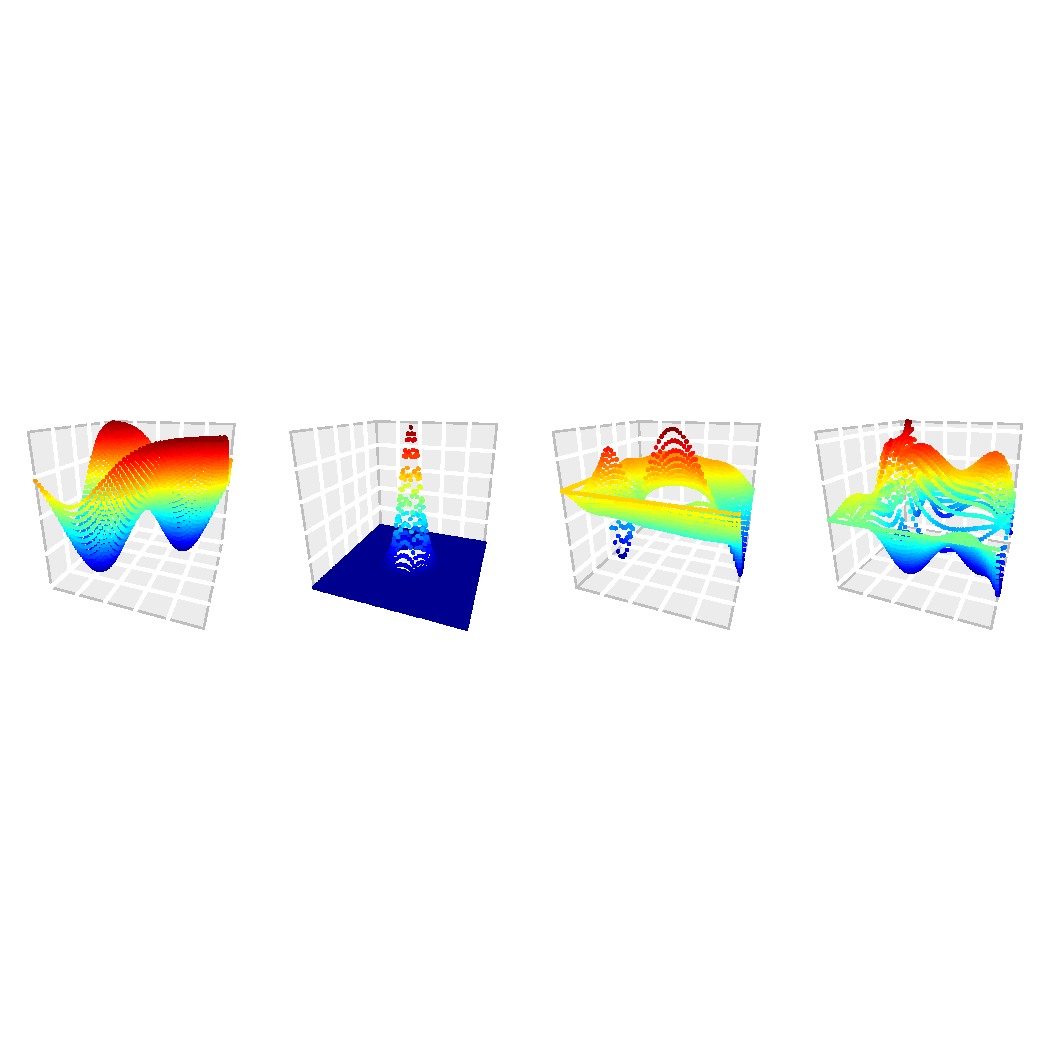
\includegraphics[width=1\textwidth]{Experiments/plots/crop_surface_truth.pdf}
    \caption{The ground truth in surface spline regression for Cases $2.1-2.4$. Cases 2.1 and 2.2 are continuous, whereas Cases 2.3 and 2.4 are discontinuous.}
    \label{fig:surface_truth}
\end{figure}
\fi

The mean squared errors are summarized in Table \ref{tab:surface}. Three EBARS versions with $\gamma=1,0.5,0$ are implemented to demonstrate the effect of $\gamma$. In Cases 2.1 and 2.2, the performance of all five methods is satisfactory and MSE of TPS is roughly the smallest. This indicates that five spline approaches do well in fitting smooth surfaces. However, when the surface is discontinuous, the prediction performance of TPS is worse than free knot splines. For example, the MSE of TPS are much larger than that of EBARS and BARS in Cases 2.3 and 2.4. BARS achieves close results to EBARS except for Case 2.4. As $k$ has to be large enough to fit Case 2.4, the performance of BARS is limited owing to the poor property of BIC in high dimension. Besides, EBARS performs slightly better with low $\gamma$ than with high $\gamma$ even in smooth cases, different from curve regression. It seems that surface regression is more likely to be underfitting rather than overfitting.

\begin{table}
\caption{MSE on test data of five methods in Cases $2.1-2.4$}
\label{tab:surface}
\centering
\begin{tabular}{cccccc}
\toprule
Methods & m                     & Case 2.1     & Case 2.2     & Case 2.3     & Case 2.4     \\
\midrule
EBARS $\gamma=1$   & \multirow{5}{*}{500}  & 0.163(0.044) & 0.624(0.107) & 0.664(0.216) & 1.133(0.443) \\
EBARS $\gamma=0.5$  &                       & 0.148(0.038) & 0.616(0.111) & 0.597(0.192) & 1.101(0.287) \\
EBARS  $\gamma=0$ &                       & 0.138(0.042) & 0.609(0.089) & 0.568(0.136) & 1.076(0.269) \\
BARS    &                       & 0.169(0.050) & 0.671(0.160) & 0.660(0.199) & 1.968(0.485) \\
TPS     &                       & 0.102(0.031) & 0.587(0.092) & 1.958(0.625) & 2.324(0.466) \\
\midrule
EBARS $\gamma=1$  & \multirow{5}{*}{1000} & 0.064(0.011) & 0.355(0.051) & 0.230(0.061) & 0.331(0.077) \\
EBARS $\gamma=0.5$  &                       & 0.066(0.016) & 0.326(0.056) & 0.222(0.053) & 0.343(0.078) \\
EBARS $\gamma=0$  &                       & 0.065(0.014) & 0.306(0.058) & 0.242(0.067) & 0.336(0.058) \\
BARS    &                       & 0.107(0.027) & 0.416(0.094) & 0.313(0.074) & 1.020(0.510) \\
TPS     &                       & 0.057(0.015) & 0.319(0.032) & 1.205(0.215) & 1.379(0.214) \\
\bottomrule
\end{tabular}
\end{table}

To graphically illustrate the difference in surface spline regression, we visualize the prediction results with $m=1000$ by contour maps in Figure \ref{fig:surface}. Initially, the fitted contours approximately overlap with the ground truth in Cases 2.1 and 2.2, see the top $2$ rows. We can see from the $(3,6)$ and $(4,6)$ panels that TPS fails to estimate the jump discontinuity in Cases 2.3 and 2.4. Actually, the fitted surfaces by TPS are always smooth regardless of the smoothness of true models. BARS obtains a nice performance in Cases 2.1-2.3, but is trapped in Case 2.4 when the required $k$ is enormous. Conversely, Columns $2-4$  of Figure \ref{fig:surface} show that our EBARS makes precise predictions in all cases successfully.

\begin{figure}
    \centering
    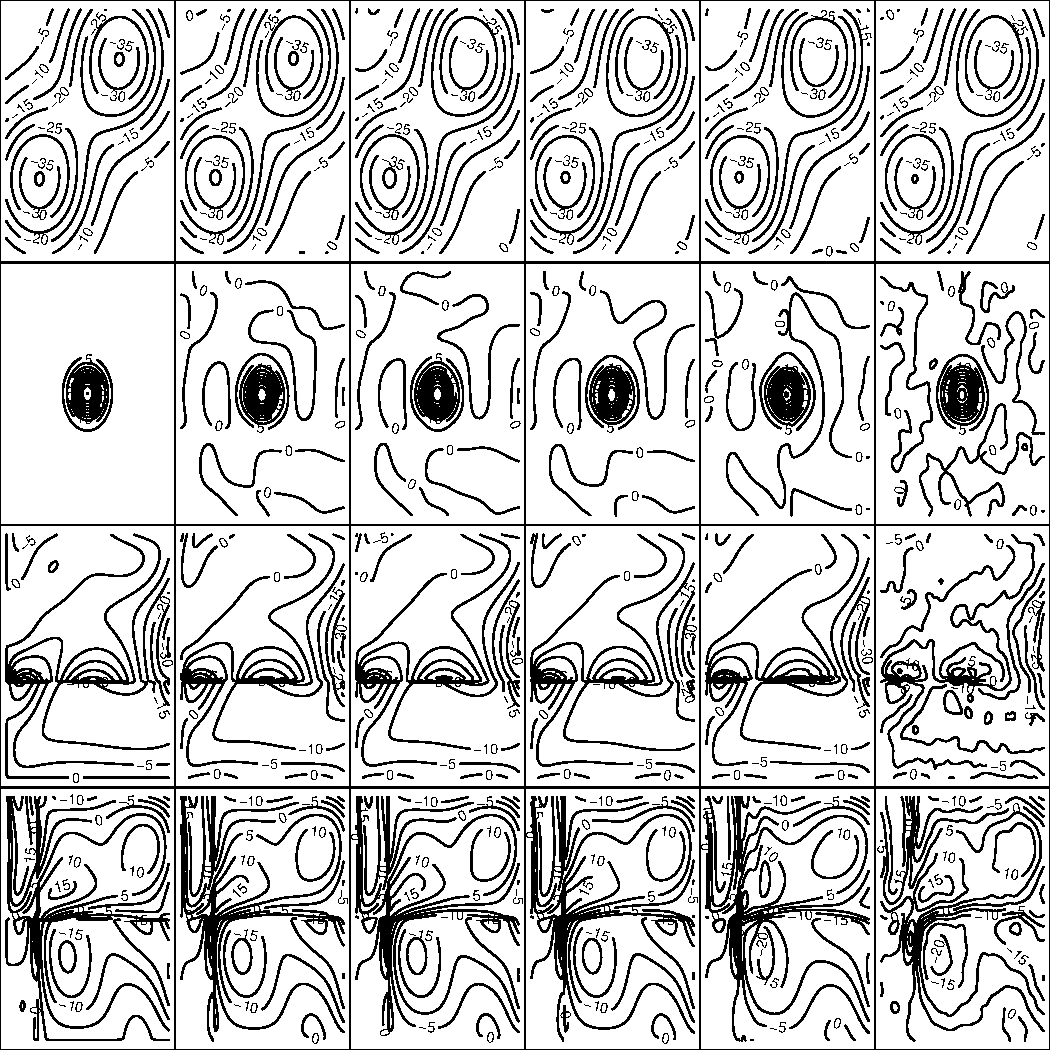
\includegraphics[width=0.85\textwidth]{Experiments/plots/surface_regression.pdf}
    \caption{Surface spline regression. It illustrates the prediction results with $m=1000$ in Cases $2.1-2.4$ by contours. From left to right, columns are respectively the ground truth, prediction by EBARS with $\gamma=1,0.5,0$, prediction by BARS and prediction by TPS.}
    \label{fig:surface}
\end{figure}